\documentclass[tikz,border=7pt]{standalone}
\begin{document}
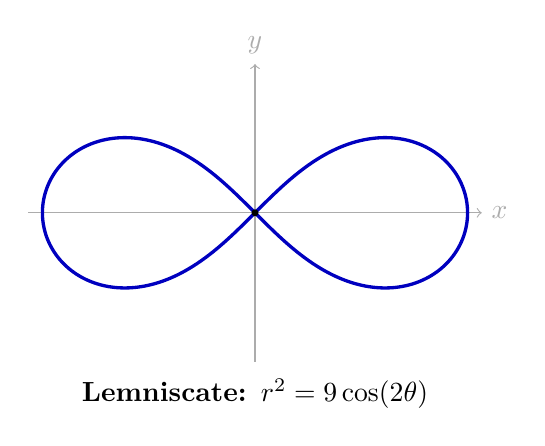
\begin{tikzpicture}[scale=.9]
\draw[->,gray!65] (-3.2,0)--(3.2,0) node[right] {$x$};
\draw[->,gray!65] (0,-2.1)--(0,2.1) node[above] {$y$};
\draw[blue!75!black,very thick,samples=400,domain=0:360,smooth,variable=\t]
  plot ({3*cos(\t)/(1+sin(\t)*sin(\t))},{3*sin(\t)*cos(\t)/(1+sin(\t)*sin(\t))});
\fill (0,0) circle (1.4pt);
\node[font=\bfseries] at (0,-2.55) {Lemniscate: $r^2=9\cos(2\theta)$};
\end{tikzpicture}
\end{document}
